% Format teze zasnovan je na paketu memoir
% http://tug.ctan.org/macros/latex/contrib/memoir/memman.pdf ili
% http://texdoc.net/texmf-dist/doc/latex/memoir/memman.pdf
% 
% Prilikom zadavanja klase memoir, navedenim opcijama se podešava 
% veličina slova (12pt) i jednostrano štampanje (oneside).
% Ove parametre možete menjati samo ako pravite nezvanične verzije
% mastera za privatnu upotrebu (na primer, u b5 varijanti ima smisla 
% smanjiti 
\documentclass[12pt,oneside]{memoir}

% Paket koji definiše sve specifičnosti mastera Matematičkog fakulteta
\usepackage{matfmaster/matfmaster}

% Linkovi u PDF-u bez crvenih/plavih okvira (ref, sadržaj, URL)
\hypersetup{
  colorlinks=true,
  linkcolor=black,
  citecolor=black,
  urlcolor=black,
  pdfpagemode=UseOutlines,
}
%
% Podrazumevano pismo je ćirilica.
%   Ako koristite pdflatex, a ne xetex, sav latinički tekst na srpskom jeziku
%   treba biti okružen sa \lat{...} ili \begin{latinica}...\end{latinica}.
%
% Opicija [latinica]:
%   ako želite da pišete latiniciom, dodajte opciju "latinica" tj.
%   prethodni paket uključite pomoću: \usepackage[latinica]{matfmaster}.
%   Ako koristite pdflatex, a ne xetex, sav ćirilički tekst treba biti
%   okružen sa \cir{...} ili \begin{cirilica}...\end{cirilica}.
%
% Opcija [biblatex]:
%   ako želite da koristite reference na više jezika i umesto paketa
%   bibtex da koristite BibLaTeX/Biber, dodajte opciju "biblatex" tj.
%   prethodni paket uključite pomoću: \usepackage[biblatex]{matfmaster}
%
% Opcija [b5paper]:
%   ako želite da napravite verziju teze u manjem (b5) formatu, navedite
%   opciju "b5paper", tj. prethodni paket uključite pomoću: 
%   \usepackage[b5paper]{matfmaster}. Tada ima smisla razmisliti o promeni
%   veličine slova (izmenom opcije 12pt na 11pt u \documentclass{memoir}).
%
% Naravno, opcije je moguće kombinovati.
% Npr. \usepackage[b5paper,biblatex]{matfmaster}

% Pomoćni paket koji generiše nasumičan tekst u kojem se javljaju sva slova
% azbuke (nema potrebe koristiti ovo u pravim disertacijama)
\usepackage{pangrami}

% Ostali paketi koji se koriste u dokumentu
\usepackage{listings} % listing programskog koda
\usepackage{array} % vertikalno poravnanje u tabelama (m{...} kolone)

% Datoteka sa literaturom u BibTex tj. BibLaTeX/Biber formatu
\bib{literatura}

\autor{Лазар Савић}
\naslov{Развој софтвера за откривање молекулских структура са потенцијално лековитим дејством}
\godina{2026}
\mentor{проф. др Јована \textsc{Ковачевић}, редован професор\\ Универзитет у Београду, Математички факултет}
\komisijaA{др Мирјана \textsc{Маљковић Ружичић}, ванредни професор\\ Универзитет у Београду, Математички факултет}
\komisijaB{Стефан \textsc{Капунац}, асистент\\ Универзитет у Београду, Математички факултет}
% Datum odbrane (obrisati ili iskomentarisati narednu liniju ako datum odbrane nije poznat)
% \datumodbrane{15. јануар 2016.}

% Apstrakt na srpskom jeziku (u odabranom pismu)
\apstr{%
Развој нових лекова представља сложен процес који захтева значајне временске и финансијске ресурсе. Примена метода рачунарске интелигенције омогућава аутоматизацију и оптимизацију појединих корака у процесу откривања нових лековитих једињења, чиме се смањује потреба за испитивањем великог броја молекула традиционалним експерименталним приступима.

У овом раду представљен је развој софтверског система за генерисање, евалуацију и оптимизацију молекулских структура са потенцијално лековитим дејством. Као основни приступ за претраживање простора могућих молекула коришћени су генетски алгоритми, уз примену различитих функција погодности за процену квалитета генерисаних структура. Систем омогућава примену оператора селекције, мутације и рекомбинације, као и праћење и анализу процеса оптимизације.

За развој система коришћен је програмски језик Python. Графички кориснички интерфејс реализован је употребом библиотеке PyQt, док је за обраду и анализу молекулских структура коришћена библиотека RDKit. За тестирање система коришћени су подаци из јавно доступне базе биоактивних молекула ChEMBL.

Развијени систем представља пример примене рачунарске интелигенције у области рачунарски потпомогнутог откривања лекова и омогућава ефикасније претраживање простора молекулских структура у циљу идентификације потенцијалних кандидата за даља фармаколошка истраживања.
}

% Ključne reči na srpskom jeziku (u odabranom pismu)
\kljucnereci{рачунарска интелигенција, генетски алгоритми, откривање лекова, молекулске структуре}

\begin{document}
% ==============================================================================
% Uvodni deo teze
\frontmatter
% ==============================================================================
% Naslovna strana
\naslovna
% Strana sa podacima o mentoru i članovima komisije
\komisija
% Strana sa posvetom (u odabranom pismu)
\posveta{Породици}
% Strana sa podacima o disertaciji na srpskom jeziku
\apstrakt
% Sadržaj teze
\tableofcontents*

% ==============================================================================
% Glavni deo teze
\mainmatter
% ==============================================================================

% ------------------------------------------------------------------------------
\chapter{Увод}
% ------------------------------------------------------------------------------


\section{Примери коришћења класичних \LaTeX{} елемената}
% primeri citiranja
Ово је реченица у којој се јавља цитат \cite{PetrovicMikic2015}.
Још један цитат \cite{GuSh:243}.
% primeri navodnika
Испробавамо наводнике: "Рекао је да му се јавимо сутра".
% primer referisanja na tabelu (koja se javlja kasnije)
У табели \ref{tbl:rezultati} која следи приказани су резултати експеримента.
% primer kraćeg latiničkog teksta
{\lat Ovo je primer rečenice ispisane latiničkim pismom u okviru ćiriličkog dokumenta.}
У овој реченици се налази једна {\lat reč} написана латиницом.
% primer korišćenja fusnota
Иза ове реченице следи фуснота.\footnote{Ово је фуснота.}
% primer url-a
Сајт математичког факултета је \url{http://www.matf.bg.ac.rs}.

% primer dužeg latiničkog teksta
\begin{latinica}
  Ovo je malo duži blok teksta ispisan latiničkim pismom u okviru
  ćiriličkog dokumenta. Fijuče vetar u šiblju, ledi pasaže i kuće iza
  njih i gunđa u odžacima.
\end{latinica}

% primer korišćenja tabele
\begin{table}
\centering
\caption{Резултати}
\label{tbl:rezultati}
\begin{tabular}{c>{\centering}p{2cm}c}
\toprule
1 & 2 & 3\\\midrule
4 & 5 & 6\\\cmidrule(rl){1-2}
7 & 8 & 8\\
\bottomrule
\end{tabular}
\end{table}

% primer korišćenja slike
\begin{figure}[!ht]
  \centering
  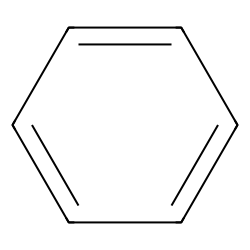
\includegraphics[width=0.5\textwidth]{slike/Benzen.png}
  \caption{Графикон}
  \label{fig:grafikon}
\end{figure}

% primer jednostavnije matematičke formule
Ево и један пример математичке формуле: $e^{i\pi} + 1 = 0$. 
% primer referisanja na sliku
На слици \ref{fig:grafikon} приказан је један графикон.

% primer kompleksnije matematičke formule
$$
\int_a^b f(x)\ \mathrm{d}x \ =_{def}\ \lim_{\max{\Delta x_k \rightarrow 0}} \sum_{k=1}^n f(x_k^*)\Delta x_k
$$

% primer referisanja na poglavlja i strane poglavlja
Више детаља биће дато у глави \ref{chp:razrada} на страни \pageref{chp:razrada}.

% primer listinga koda

У тезу можемо убацити и програмски кôд.

\begin{verbatim}
Ovo je doslovni tekst.
\end{verbatim}

\begin{english}
\lstset{
  language=C,
  basicstyle=\ttfamily,
  keywordstyle=\color{blue}
}
\begin{lstlisting}
#include <stdio.h>

int main() {
   printf("Hello, world!\n");
   return 0;
}
\end{lstlisting}
\end{english}


Овај C програм се може превести помоћу преводиоца GCC \cite{gcc}.

% primer liste
Можемо правити и набрајања:
\begin{enumerate}
\item Анализа 1
\item Линеарна алгебра
\item Аналитичка геометрија
\item Основи програмирања
\end{enumerate}

% ------------------------------------------------------------------------------
\chapter{Репрезентација молекула у програмима}
\label{chp:2}
% ------------------------------------------------------------------------------
Молекулске структуре могу се представити на више различитих начина, при чему свака репрезентација наглашава одређене аспекте молекула и прилагођена је конкретној намени. Док су неке репрезентације погодне за једноставно записивање и размену података о молекулима, друге омогућавају њихову рачунарску обраду, анализу или примену у алгоритмима машинског учења. Избор одговарајуће репрезентације зависи од проблема који се решава и операција које је потребно извршити над молекулским структурама.

У овом раду коришћене су три међусобно повезане репрезентације молекула. За текстуални запис молекулских структура коришћена је SMILES нотација \ref{chp:smiles}, за њихову интерну репрезентацију и манипулацију библиотека RDKit користи објекат типа Mol \ref{chp:rdkit-mol}, док су за потребе обучавања модела машинског учења и предикције биолошке активности молекули представљени помоћу Morgan fingerprint вектора \ref{chp:mf-vec}. У наставку су описане основне карактеристике сваке од наведених репрезентација и њихова улога у оквиру развијеног система.


\section{SMILES нотација}
\label{chp:smiles}

SMILES (енг. \textit{Simplified Molecular Input Line Entry System}) \cite{Weininger1988} представља једноставан и компактан текстуални начин представљања молекулских структура у облику ниске ASCII карактера. Због своје читљивости и мале величине записа, широко се користи за складиштење, размену и обраду података о молекулима. Иако је реч о једнодимензионом текстуалном запису, SMILES омогућава представљање структуре молекула, укључујући атоме, хемијске везе, гранања и цикличне структуре, а по потреби и информације о стереохемији. Заснива се на неколико једноставних правила записа, која ће у наставку бити описана и илустрована примерима датим у табели \ref{tab:smiles_examples}.

\textbf{Правило 1 - Атоми:} Атоми који улазе у састав молекула представљени су својим хемијским симболима, у угластим заградама. Ове заграде се изостављају за "органски" подскуп атома - B, C, N, O, P, S, F, Cl, Br и I. Ако су заграде изостављене, подразумеван је имплицитан број водоникових атома који задовољава стандардну валенцу атома, те се у тим случајевима H атоми изостављају. Јони се увек пишу у заградама, попут $\mathrm{[Co^{3+}]}$ или $\mathrm{[OH^{-}]}$. 

\textbf{Правило 2 - Везе:} Везе између атома представљају се на различите начине, у зависности од њихове вишеструкости. Везе између суседних атома су подразумевано једноструке, и тада се оне не наводе. Двоструке везе представљене су симболом '=', а троструке са '\#'. Ароматичне везе могу се експлицитно представити симболом ':'.

\textbf{Правило 3 - Гранања:} У случају разгранатих молекула, грана која се издваја из родитељског ланца је одвојена обичним заградама '()'.

\textbf{Правило 4 - Циклуси:} Циклични молекули се такође записују линеарно, тако што се позиције на којима се прстен отвара и затвара обележе истим бројем. У случају ароматичних прстена, сви атоми који учествују у том прстену обележавају се малим словима, како би се разликовали од одговарајућих алифатичних прстена.

\textbf{Правило 5 - Неповезане структуре:} Уколико се молекул састоји од више неповезаних компоненти, он се може представити тако што се на сваку компоненту примене правила 1 - 4, и добијени записи се повежу симболом '.'.

\begin{table}[h]
\centering
\begin{tabular}{|>{\centering\arraybackslash}m{2.4cm}|>{\centering\arraybackslash}m{3.2cm}|>{\centering\arraybackslash}m{2.4cm}|}
\hline
\textbf{Молекул} & \textbf{Структура} & \textbf{SMILES} \\
\hline
Етанол & 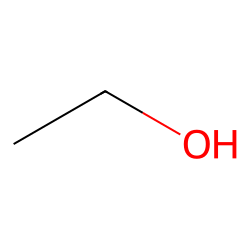
\includegraphics[height=1.6cm]{slike/Etanol.png} & \texttt{CCO} \\
\hline
Етен & 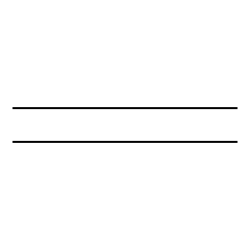
\includegraphics[height=1.6cm]{slike/Eten.png} & \texttt{C=C} \\
\hline
Изобутан & 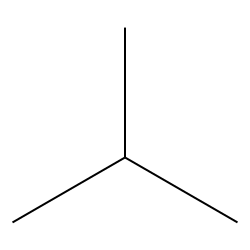
\includegraphics[height=1.6cm]{slike/Izobutan.png} & \texttt{CC(C)C} \\
\hline
Бензен & 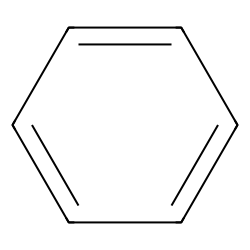
\includegraphics[height=1.6cm]{slike/Benzen.png} & \texttt{c1ccccc1} \\
\hline
\end{tabular}
\label{tab:smiles_examples}
\caption{Примери молекулских структура и одговарајућих SMILES записа}
\end{table}

Важно је напоменути да SMILES запис није јединствен за један молекул. Иста молекулска структура може имати више различитих SMILES записа, у зависности од избора почетног атома и редоследа обиласка структуре. Како би се обезбедила јединствена и стандардизована репрезентација молекула, често се користи канонски SMILES запис, који алгоритамски одређује један представник за дату молекулску структуру.

\section{Објекат Mol библиотеке RDKit}
\label{chp:rdkit-mol}

RDKit (енг. \textit{RDKit Cheminformatics Toolkit}) је open-source библиотека за рад са молекулским 
структурама \cite{Landrum2006}. Имплементирана је у C++-у, са Python интерфејсом, и широко се користи 
у областима попут хемоинформатике и машинског учења \footnote{Поготово у комбинацији ове две области - 
компјутерски потпомогнуто откривање лекова, што је и суштина овог рада.}. За разлику од текстуалних 
формата попут SMILES-a, RDKit пружа богат интерфејс за рад са молекулима, кроз објекат \texttt{Mol}. 
Објекат \texttt{Mol} интерно представља молекулску структуру као граф чији су чворови атоми, а гране хемијске везе, уз додатне информације о особинама веза и атома. Оваква репрезентација омогућава ефикасно извршавање различитих операција 
над молекулима, као што су валидација структуре, израчунавање молекулских дескриптора, 
генерисање Morgan fingerprint вектора, као и визуализацију структура у корисничком интерфејсу.

\section{Morgan fingerprint вектори}
\label{chp:mf-vec}

Morgan fingerprint \cite{RogersHahn2010} представља нумеричку репрезентацију молекулске структуре у облику 
бит-вектора фиксне дужине, погодну за примену алгоритама машинског учења. За разлику 
од SMILES записа и RDKit Mol објекта, који чувају информације о структури молекула, 
Morgan fingerprint издваја присуство одређених локалних структурних карактеристика
молекула и кодира их у бинарни вектор. На тај начин сваки бит представља присуство 
или одсуство одређеног структурног мотива, што омогућава једноставну примену математичких 
и машинских метода над молекулским подацима (слика \ref{fig:morgan-fingerprint}).

\begin{figure}[!ht]
  \centering
  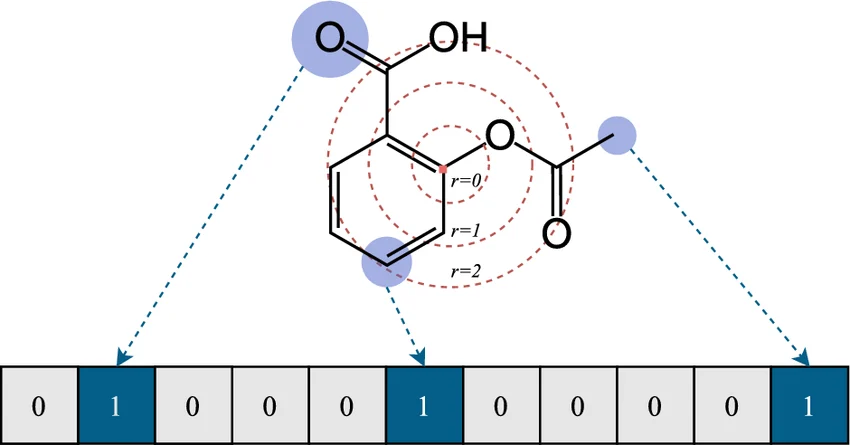
\includegraphics[width=\textwidth]{slike/MorganFingerprint.png}
  \caption{Пример Morgan fingerprint репрезентације (аспирин): бит-вектор и подструктуре за различите радијусе. Преузето из \cite{NguyenVo2024}.}
  \label{fig:morgan-fingerprint}
\end{figure}

Генерисање Morgan fingerprint вектора заснива се на итеративном обиласку околине сваког 
атома у молекулу. За сваки атом посматрају се суседни атоми до задатог растојања, 
дефинисаног параметром \textit{radius}, након чега се добијене локалне структуре хеширају 
и пресликавају у позиције бит-вектора.
Избор вредности овог параметра представља компромис између детаљности и 
генерализације молекулске репрезентације. Мање вредности описују локалне карактеристике 
блиске појединачним атомима, док веће омогућавају кодирање сложенијих 
структурних фрагмената који обухватају већи део молекула.


% ------------------------------------------------------------------------------
\chapter{Предикција биолошке активности}
\label{chp:models}
% ------------------------------------------------------------------------------

У оквиру развијеног система потребно је проценити потенцијалну биолошку активност генерисаних молекулских структура како би се омогућило њихово рангирање у оквиру генетског алгоритма. Пошто експериментално одређивање активности сваке новогенерисане структуре није могуће у току процеса оптимизације, развијени су предиктивни модели који представљају брзе рачунарске апроксимације експерименталних мерења.

За потребе обучавања модела коришћени су подаци из јавно доступне базе биоактивних молекула ChEMBL. Изабране су молекулске структуре за које постоје експериментално одређене вредности активности према циљном протеину EGFR (\textit{Epidermal Growth Factor Receptor}). Основна вредност која се у овом раду предвиђа је IC50 (\textit{half maximal inhibitory concentration}), која представља концентрацију супстанце потребну за постизање 50\% инхибиције одређеног биолошког процеса. Ниже вредности IC50 указују на већу потентност молекула, па се у циљу погодније примене у моделима машинског учења често користи трансформисана вредност pIC50, при чему је $\textrm{pIC50} = -\log_{10}(\textrm{IC50})$.

Молекулске структуре из одабраног скупа представљене су помоћу Morgan fingerprint вектора, који су коришћени као улазни атрибути различитих регресионих модела за предикцију pIC50 вредности. Обучени модели затим служе као заменски модели (\textit{surrogate models}) у оквиру генетског алгоритма, где омогућавају процену фитнес функције новогенерисаних молекула без потребе за експерименталним мерењем њихове биолошке активности.

\section{Претпроцесирање података}
\label{sec:preprocessing}

\section{Припрема улазних одлика}
\label{sec:feature-prep}

\section{Подела на обучавајући, валидациони и тест скуп}
\label{sec:train-val-test-split}

\section{Предиктивни модели}
\label{sec:predictive-models}

\subsection{Ridge регресија}
\label{sec:model-ridge}

\subsection{Random Forest}
\label{sec:model-rf}

\subsection{LightGBM}
\label{sec:model-lgbm}

\section{Оптимизација хиперпараметара}
\label{sec:hyperparam-tuning}

\section{Резултати и упоредна анализа}
\label{sec:model-results}

\section{Избор модела за коришћење у систему}
\label{sec:model-selection}


% ------------------------------------------------------------------------------
\chapter{Развој софтверске апликације}
\label{chp:razrada}
% ------------------------------------------------------------------------------

% ------------------------------------------------------------------------------
\chapter{Генетски алгоритам}
% ------------------------------------------------------------------------------

\section{Јединке и популација}

\section{Фитнес функција}

\section{Селекција}

\section{Укрштање}

\section{Мутација}

% ------------------------------------------------------------------------------
\chapter{Експериментални резултати}
% ------------------------------------------------------------------------------

% ------------------------------------------------------------------------------
\chapter{Дискусија}
% ------------------------------------------------------------------------------

% ------------------------------------------------------------------------------
\chapter{Закључак}
% ------------------------------------------------------------------------------

% ------------------------------------------------------------------------------
% Literatura
% ------------------------------------------------------------------------------
\literatura

% ==============================================================================
% Završni deo teze i prilozi
\backmatter
% ==============================================================================

% ------------------------------------------------------------------------------
% Biografija kandidata
\begin{biografija}
\textbf{Вук Стефановић Караџић} (\emph{Тршић, 26. октобар/6. новембар
  1787. — Беч, 7. фебруар 1864.}) био је српски филолог, реформатор
српског језика, сакупљач народних умотворина и писац првог речника
српског језика.  Вук је најзначајнија личност српске књижевности прве
половине XIX века. Стекао је и неколико почасних доктората.
Учествовао је у Првом српском устанку као писар и чиновник у
Неготинској крајини, а након слома устанка преселио се у Беч,
1813. године. Ту је упознао Јернеја Копитара, цензора словенских
књига, на чији је подстицај кренуо у прикупљање српских народних
песама, реформу ћирилице и борбу за увођење народног језика у српску
књижевност. Вуковим реформама у српски језик је уведен фонетски
правопис, а српски језик је потиснуо славеносрпски језик који је у то
време био језик образованих људи. Тако се као најважније године Вукове
реформе истичу 1818., 1836., 1839., 1847. и 1852.
\end{biografija}
% ------------------------------------------------------------------------------

\end{document} 